%! Author = Frederik Bußmann
%! Date = 22.06.2023

\section{Analyse und Konzept} \label{sec:03-concept}

Im folgenden Kapitel werden verschiedene Techniken zur kontinuierlichen Integrierung von Code analysiert und eine
Konzeption für Shopware-basierte Projekte erarbeitet.
Zunächst werden technische Anforderungen an die zu entwickelnde Strategie im Hinblick auf die geschäftsseitigen
Vorgaben durch die Ziele $Z_n$ der Arbeit definiert.
Anschließend wird die Ausgangssituation in Shopware-Projekten und dessen Umgebungen und kundenspezifischer Anpassungen
beleuchtet, wobei der Fokus auf den gemeinsamen Grundvoraussetzungen und der Anpassungsfähigkeit der
\acrshort{ci}-Strategie an verschiedene Architekturen liegt.
Zuletzt wird die eigentliche Konzeption der Strategie anhand der zuvor erarbeiteten Methoden und
Praktiken und den definierten Anforderungen vorgenommen.

\subsection{Technische Anforderungen} \label{subsec:03-concept-1}

Um ein vollumfängliches Konzept erstellen zu können, müssen einige technische Anforderungen an die Strategie definiert
werden.
Diese Anforderungen orientieren sich sowohl an der Zieltechnologie – in diesem Fall Shopware – als auch an den im
fachlichen Hintergrund erörterten Methoden und Praktiken.
Da die Strategie das Nutzen von\ \acrshort{ci} in Shopware-Projekten ermöglichen soll, werden nachfolgend
die technischen Anforderungen an das Konzept im Hinblick auf die Gegebenheiten der Shop-Software aufgezeigt:

\begin{itemize}
    \item {
        \textbf{Vollautomatisierter Software-Build}\par
        Der Prozess des Software-Builds muss durchweg automatisiert stattfinden.
        Dies umfasst das Installieren der Software aus der Versionskontrolle, dem Herunterladen und Installieren
        sämtlicher Abhängigkeiten und dem Erzeugen von Build-Dateien aus dem gegebenen Quellcode.
    }

    \item {
        \textbf{Automatisierte Software-Tests und Quality-Checks}\par
        Da Testing einen integralen Bestandteil der\ \acrshort{ci} bildet, muss die zu konzipierende Strategie ein
        umfassendes Test-Konzept bieten.
        Dies schließt sowohl Unit- und Module-Tests, als auch programmübergreifende Prüfungen wie Integration- und
        System-Tests ein.
        Zudem soll die Qualitätssicherung der zu entwickelnden Software eines Projekts durch statische
        Code-Analyse-Tools in die \acrshort{ci}-Strategie integriert werden.
    }

    \item {
        \textbf{Reproduzierbare\ \acrshort{ci}-Umgebungen}\par
        Es ist von entscheidender Bedeutung, dass die \acrshort{ci}-Umgebung konsistent und reproduzierbar ist.
        Dies gewährleistet, dass jeder Build und Test unter identischen Bedingungen durchgeführt wird, unabhängig davon,
        wann und wo der \acrshort{ci}-Prozess initiiert wird.
        Die Strategie sollte daher die Verwendung von Containerisierungstechnologien, wie Docker, in Betracht ziehen,
        um eine einheitliche, isolierte und wiederholbare Umgebung für den Build- und Testprozess zu schaffen.
        Dies minimiert potenzielle Inkonsistenzen und Fehler, die durch unterschiedliche Umgebungsbedingungen entstehen
        könnten.
    }

    \item {
        \textbf{Hohe Anpassbarkeit und Skalierbarkeit}\par
        Die \acrshort{ci}-Strategie sollte flexibel genug sein, um sich an veränderte Anforderungen und wachsende
        Projektgrößen anzupassen.
        Dies bedeutet, dass sowohl die Infrastruktur als auch die Prozesse skalierbar gestaltet werden müssen, um mit
        der Evolution des Projekts Schritt zu halten.
        Die Möglichkeit, neue Tools und Technologien nahtlos zu integrieren, sollte ebenfalls gegeben sein, um die
        kontinuierliche Anpassung und Optimierung der \acrshort{ci}-Pipeline zu gewährleisten.
    }

    \item {
        \textbf{Einheitliche Daten-Verwaltung}\par
        Um Konsistenz und Nachvollziehbarkeit zu gewährleisten, sollte alles, von Code über Konfigurationen bis hin
        zu Datenbank-Skripten und Tests, in einem Versionskontrollsystem verwaltet werden.
        Dies ermöglicht eine klare Historie von Änderungen und erleichtert das Rollback im Falle von Problemen.
        Ein zentralisiertes\ \acrshort{vcs} stellt sicher, dass alle Teammitglieder stets mit der aktuellsten Version
        arbeiten und Änderungen nachvollziehbar sind.
    }

    \item {
        \textbf{Kontinuierliche Bereitstellung und Deployments}\par
        Neben dem Build- und Testing-Prozess ist es auch wichtig, dass die \acrshort{ci}-Strategie Mechanismen für die
        kontinuierliche Bereitstellung und das Deployment der Software bietet.
        Dies ermöglicht es, Änderungen schnell in die Produktionsumgebung zu übertragen und sicherzustellen, dass die
        Software stets aktuell und einsatzbereit ist.
        Automatisierte Deployments sollten daher in den Pipelines mit eingeplant werden, um den Prozess der
        Softwareauslieferung zu optimieren und zu beschleunigen.
    }

    \item {
        \textbf{Hohe System-Verfügbarkeit}\par
        Die \acrshort{ci}-Infrastruktur sollte so konzipiert sein, dass sie stets verfügbar ist und minimale Ausfallzeiten
        aufweist. Dies ist entscheidend, um den kontinuierlichen Entwicklungsfluss nicht zu unterbrechen und eine
        ständige Feedback-Schleife zu gewährleisten.
        Redundanzen und regelmäßige Backups sollten implementiert werden, um die Systemverfügbarkeit auch bei
        unerwarteten Problemen zu gewährleisten.
    }
\end{itemize}

Diese technischen Anforderungen sollen das Entwickeln einer vollumfänglichen\ \acrshort{ci}-Strategie im Hinblick auf
die definierten Ziele $Z_n$ der Arbeit ermöglichen.

\subsection{Analyse der Ausgangssituation} \label{subsec:03-concept-2}

Die aktuelle Situation stellt sich wie folgt dar: In E-Commerce-Unternehmen die Shopware-Projekte betreiben, gibt es in
der Regel verschiedene Kunden, die mit unterschiedlichen Versionen von der Software arbeiten.
Diese Kunden können bei verschiedenen Hosting-Anbietern untergebracht sein, was zu einer Vielfalt an technischen
Umgebungen führt, in denen die Software betrieben wird.
Darüber hinaus verwenden Kunden meist eine individuelle Kombination aus Plugins und Eigenentwicklungen, die auf dessen
spezifische Bedürfnisse zugeschnitten sind.
Diese Diversität stellt eine Herausforderung dar, da sie eine Vielzahl von Variablen in die Entwicklung und Wartung der
Software einbringt.
Um eine generalisierte Strategie erstellen zu können, wird sich also zunächst auf die Gemeinsamkeiten von
Shopware-Projekten konzentriert.
Shopware besteht aus einer Vielzahl von Verzeichnissen und Dateien, jede Version der Software und jedes
Shopware-basierte Projekt unterscheiden sich voneinander.
Ungeachtet von Projekt und Version gibt es jedoch einige Grundvoraussetzungen für das Ausführen von Shopware.
\footpartcite{shopware-requirements}

\begin{figure}[H]
    \centering
    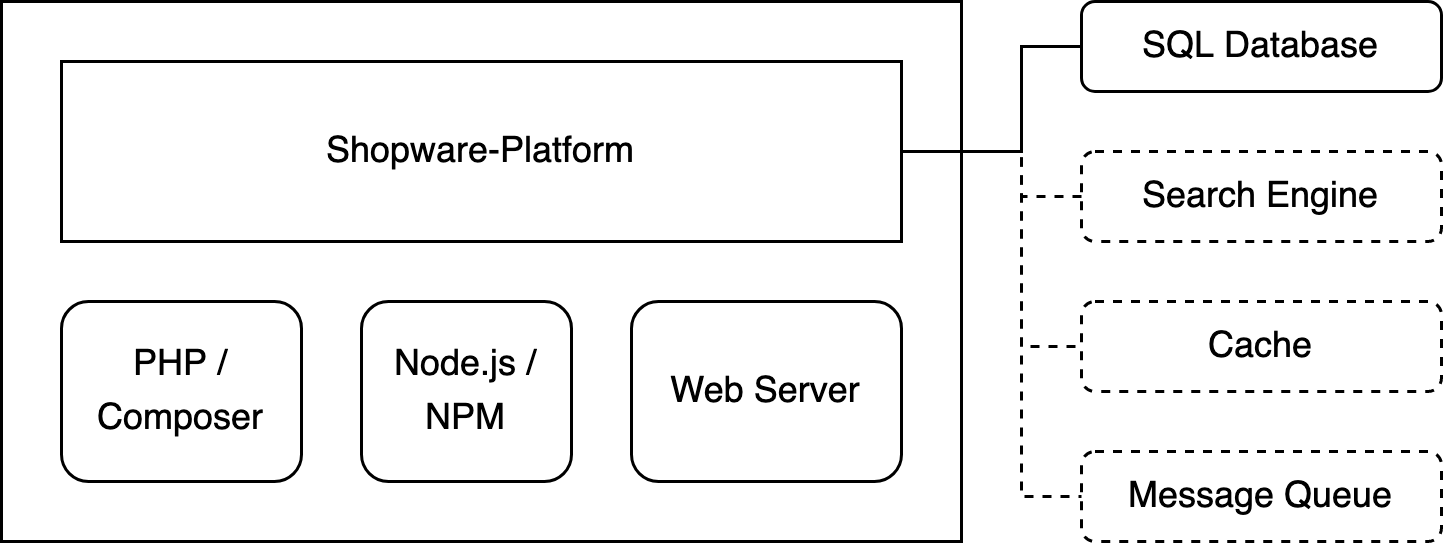
\includegraphics[width=0.75\textwidth]{images/content/shopware-requirements}
    \captioncite[Eigene Darstellung nach]{shopware-requirements}{Umgebung und Abhängigkeiten der Shopware-Platform}
    \label{fig:shopware-requirements}
\end{figure}

In Abbildung\ \ref{fig:shopware-requirements} werden die grundsätzlichen Abhängigkeiten der Shopware-Platform und die
verschiedenen Services für den Betrieb der Software aufgezeigt.
Hierbei werden optionale Services in gestrichelt dargestellt.
Um ein Projekt installieren und ausführen zu können, oder um Tests auf der Codebase durchzuführen, wird also eine
Umgebung vorausgesetzt, in der die benötigten Services und Tools installiert sind.
Nachfolgend werden die in der Grafik aufgezeigten Abhängigkeiten und Services erläutert:

\begin{itemize}
    \item {
        \textbf{PHP}\par
        Da Symfony und somit auch Shopware auf der Programmiersprache PHP basieren, muss diese in der ausführenden
        Umgebung installiert sein.

        \begin{itemize}
            \item {
                \textbf{PHP-Extensions}\par
                Shopware benötigt für den Betrieb einige PHP-Extensions, zum Beispiel zum Erstellen von Archiven
                oder dem Lesen von XML-Dateien.
            }

            \item {
                \textbf{Paketmanager\ \glqq Composer\grqq}\par
                Durch Composer werden sowohl die Abhängigkeiten von Symfony und Shopware, als auch Third-Party-Plugins
                und eigene Entwicklungen im Projekt verwaltet und zur Nutzung im PHP-Code bereitgestellt.
            }
        \end{itemize}
    }

    \item {
        \textbf{JavaScript}\par
        JavaScript bei der Nutzung der Shopware-Platform sowohl im Browser, als auch Serverseitig ausgeführt.

        \begin{itemize}
            \item {
                \textbf{JavaScript-Runtime\ \glqq Node\grqq}\par
                Zur Serverseitigen Ausführung von JavaScript-Code wird die Node-Runtime als Abhängigkeit vorausgesetzt.
            }

            \item {
                \textbf{Node-Paketmanager\ \glqq\acrshort{npm}\grqq}\par
                Der Paktemanager\ \acrshort{npm} ist eine weitere Abhängigkeit von Shopware.
                Dieser verwaltet JavaScript-Pakete, welche zur Ausführung der Software benötigt werden.
            }
        \end{itemize}
    }

    \clearpage

    \item {
        \textbf{Webserver}\par
        Um die Shop-Instanz im Browser aufrufen und\ \acrshort{api}-Anfragen verarbeiten zu können, wird eine
        Webserver-Software benötigt.
    }

    \item {
        \textbf{Datenbank}\par
        Shopware schreibt zur Nutzung der Software eine Datenbank vor, welche die eigentlichen Shop-Konfigurationen,
        Produkte, Bestellungen, Kunden und weitere Daten verwaltet.
    }

    \item {
        \textbf{Search Engine}\par
        Um den Besuchern des Online-Shops eine Textsuche für Produkte und Hersteller zu bieten, unterstützt Shopware
        das optionale Anbinden verschiedener Suchmachinen.
    }

    \item {
        \textbf{Cache}\par
        Zur Optimierung der Shop-Performance kann zudem optional ein Zwischenspeicher, auch\ \glqq Cache\grqq\ genannt,
        für Warenkorb-Inhalte und aktuelle Nutzer-Sitzungen eingeführt werden.
    }

    \item {
        \textbf{Message Queue}\par
        Um viele gleichzeitige Zugriffe von Usern verwalten zu können, erlaubt Shopware das Anbinden einer Message
        Queue.
        Diese ermöglichen das Sammeln von Nutzer-Anfragen, welche dann in Reihe verarbeitet werden können.
    }
\end{itemize}

Durch das Installieren dieser grundlegenden Abhängigkeiten und Services wird das Betreiben von Shopware 6 ermöglicht.
Da diese sich in zukünftigen Versionen der Software ändern können, sollte bei neuen Projekten immer geprüft werden,
welche Abhängigkeiten für die gewünschte Shopware-Version vorgegeben sind.
Alte Projekte sollten außerdem kontinuierlich auf aktuelle Versionen upgedatet und auf die Erfüllung von dessen
Voraussetzungen geprüft werden.

\subsection{Konzeption der CI-Strategie} \label{subsec:03-concept-3}

Im Folgenden wird die Konzeption der\ \acrshort{ci}-Strategie für Kundenprojekte auf Basis der Shopware-Platform
durchgeführt.
Hierbei wird zunächst die ausführende Umgebung geplant, sowohl für das lokale Entwickeln mit Shopware als auch für die
Integration und Ausführung der verschiedenen\ \acrshort{ci}-Tools innerhalb einer Pipeline.
Anschließend wird die Struktur der angedachten Pipeline aufgestellt, wobei dessen einzelne Aufgaben systematisch in
eigene Phasen und Jobs unterteilt werden.

\subsubsection{Projekt-Struktur und Umgebung}

Die Anforderungen des Projekts setzten eine Umgebung, in der die Shopware-Platform ausgeführt, getestet und analysiert
werden kann voraus.
Eine Umgebung muss in diesem Fall sowohl lokal als auch in einer \acrshort{ci}-Pipeline ausführbar sein und die
Grundbedürfnisse der Shopware-Instanz bereitstellen.
Dies beinhaltet die von Shopware genutzte PHP-Version mit PHP-Erweiterungen, Composer, Node, eine
Webserver-Software und weitere Voraussetzungen.
Da spätere Umgebungen, an welche die Software ausgeliefert werden soll, nicht zwangsläufig unter der
Kontrolle des Entwicklerteams stehen, wird sich in der Strategie auf die Vereinheitlichung der lokalen
Entwicklungsumgebung und der Pipeline beschränkt.
Hierzu empfiehlt sich die Nutzung von Containerization, wobei die Abhängigkeiten zum Ausführen der Shopware-Platform
und der\ \acrshort{ci}-Tools gebündelt und wiederverwendet werden können.
Ein lokal entwickeltes Feature kann so nach der Fertigstellung über ein\ \acrshort{vcs} integriert werden, welches dann
die Pipeline-Orchestration anstößt.
Die Pipeline soll zur Ausführung der einzelnen Jobs das gegebene Image instanziieren und als ausführende
Umgebung verwenden, sodass diese möglichst der lokalen Entwicklungsumgebung gleicht.
Nach dem erfolgreichen Durchlaufen des Software-Builds, Tests und Qualitäts-Checks soll die Software letztlich durch
einen Deployment-Job innerhalb der Pipeline automatisiert an verschiedene Umgebungen ausgeliefert werden können.
Hierbei kann es sich um die Produktionsumgebung oder andere Infrastrukturen handeln, wie zum Beispiel einen
Development-Server zum Testen von Features oder einen Staging-Server für die Abnahme von neuen Änderungen durch
Projekt-Kunden.

\begin{figure}[H]
    \centering
    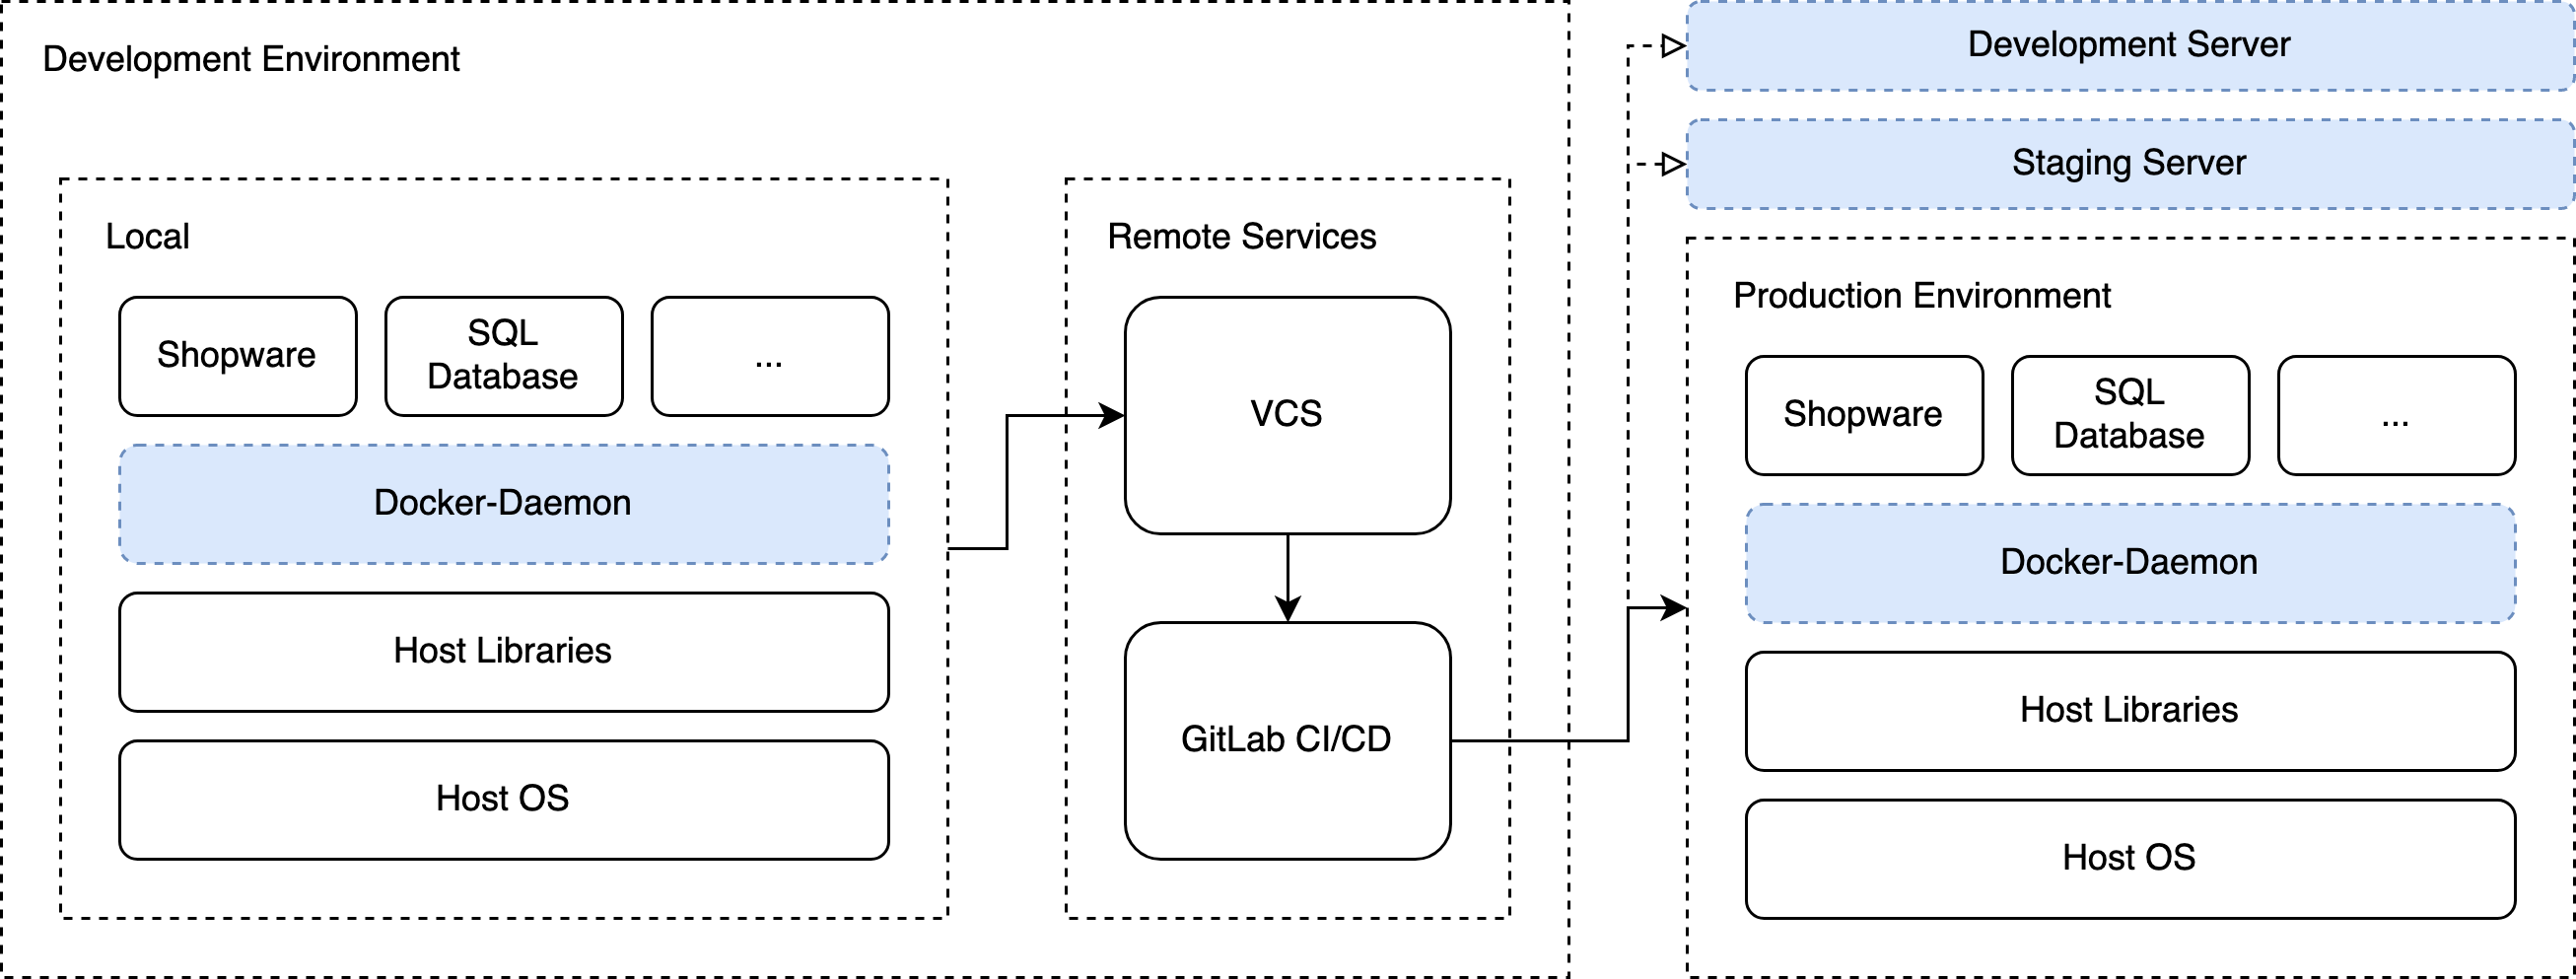
\includegraphics[width=\textwidth]{images/content/ci-architecture-concept}
    \captioncite[Eigene Darstellung nach]{docker}{Geplante Architektur der\ \acrshort{ci}-Strategie}
    \label{fig:ci-architecture-concept}
\end{figure}

Eine Visualisierung der geplanten Architektur für die\ \acrshort{ci}-Strategie kann in
Abbildung\ \ref{fig:ci-architecture-concept} eingesehen werden.
Die Darstellung zeigt die Struktur der lokalen Entwicklungsumgebung so wie der späteren möglichen
Deployment-Umgebungen in Zusammenhang mit dem\ \acrshort{vcs} und des Pipeline-Runners auf.
Optionale Services und Umgebungen werden in Blau dargestellt, der Lebenszyklus von Integrationen in der Strategie wird
durch die Pfeile zwischen den Teilbereichen verdeutlicht.
Die lokale und die Deployment-Umgebungen basieren dabei auf Hardware-Ressourcen, auf denen jeweils ein
Betriebssystem (Host\ \acrshort{os}) installiert ist, welches das Nutzen von Host Libraries ermöglicht.
Als Host Libraries werden in diesem Fall die installierten Programme und Services auf dem Betriebssystem bezeichnet,
welche zum Beispiel für das Ausführen des Docker-Daemons und dessen Containern oder für das direkte Ausführen der
Shopware-Services und dessen Abhängigkeiten genutzt werden.

\subsubsection{Aufbau der Pipeline}

Im Mittelpunkt der\ \acrshort{ci}-Strategie steht die Pipeline zum automatischen Bauen, Testen und Ausliefern der
Software.
Nachdem die Umgebung für Projekte und der grundsätzliche Ablauf von Integrationen in der Strategie definiert wurde, wird
nun die eigentliche Pipeline entworfen.
Da diese Pipeline verschiedene Phasen durchläuft, werden nachfolgend die für die Strategie angedachten Stages und dessen
Aufbau erläutert.

\begin{itemize}
    \item {
        \textbf{Build-Stage}\par
        Ungeachtet der späteren ausführenden Umgebung muss in einem Shopware-Projekt zur Durchführung weiterer Schritte
        eine Build-Phase durchlaufen werden.
        Hierbei werden die Abhängigkeiten der Shopware-Platform selbst, zusammen mit weiteren Paketen wie Testing- und
        \acrshort{qa}-Tools installiert und somit für die Testing-Phase vorbereitet.
        Die hierbei stattfindende Integration wird also zunächst durch den Status des Software-Builds geprüft.
        Ist der Build-Job erfolgreich, wird ein Artifact erzeugt welches, um die Durchlaufzeit der Pipeline insgesamt
        möglichst gering zu halten, in einem Cache zur weiteren Nutzung zwischengespeichert wird.
    }

    \item {
        \textbf{Test-Stage}\par
        Wenn die Build-Stage erfolgreich durchgelaufen ist und ein Artifact erzeugt wurde, beginnt die Testing-Phase.
        In der Strategie ist hierbei das parallele Ausführen von Tests und\ \acrshort{qa}-Tools auf der bestehenden
        Codebase angedacht.
        Um Tests parallel auszuführen werden mehrere Jobs gestartet, welchen bereits alle installierten Tools
        und der zu testende Quellcode durch das zwischengespeicherte Artifact des Build-Jobs zur Verfügung stehen.
        Hierbei sollte eine möglichst große Abdeckung des Codes durch verschiedene Arten von Software-Tests bestehen.
        Durch Unit-, Module- und Integration-Tests kann an dieser Stelle die Funktionalität der einzelnen
        Anwendungs-Komponenten überprüft werden, während System-Tests die Korrektheit des Gesamtsystems anhand der
        Geschäftsanforderungen abdecken.
        Besondere Anforderungen einzelner Testing-Tools, wie zum Beispiel ein Datenbank-Service innerhalb der Pipeline
        zum Ausführen von System-Tests, sollten dabei nicht in der Build-Phase, sondern vor der Ausführung des Tools im
        jeweiligen Job installiert werden.
        Parallel zu den verschiedenen Test-Arten können in diesem Schritt Tools zur Static-Code-Analysis ausgeführt
        werden.
        Die Test-Stage umfasst somit die automatisierte Qualitäts- und Funktionalitäts-Prüfung der Shop-Software in der
        \acrshort{ci}-Pipeline.
    }

    \item {
        \textbf{Deployment-Stage}\par
        Wenn der Software-Build inklusive aller automatisierten Tests und Qualitäts-Checks erfolgreich durchlaufen,
        kann eine Deployment-Stage gestartet werden.
        In der Strategie ist dessen Ausführung für Branches angedacht, bei denen eine Ziel-Umgebung zur Auslieferung
        des gebauten Artifacts existiert, wie zum Beispiel die Produktionsumgebung.
        Der hierbei ausgeführte Deployment-Job liefert die relevanten Daten der Shop-Software, exklusive Testing-Tools
        und\ \acrshort{ci}-Abhängigkeiten, an die definierte Umgebung aus.
        Hierbei muss beachtet werden, dass die Ausfallzeit der Applikation bei der automatischen Auslieferung so gering
        wie möglich bleibt, um die technischen Anforderungen der Strategie zu erfüllen.
    }
\end{itemize}



\begin{figure}[H]
    \centering
    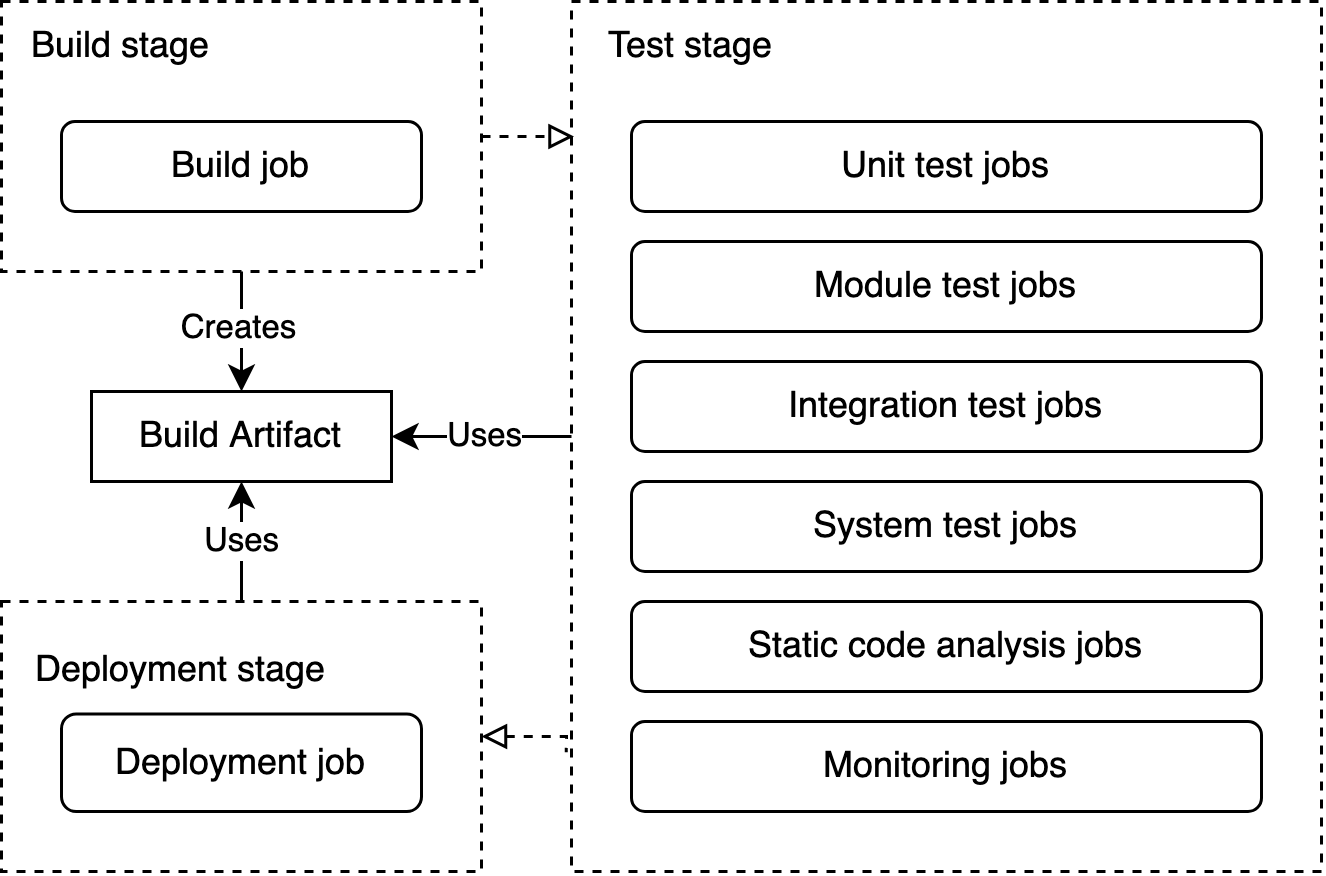
\includegraphics[width=0.75\textwidth]{images/content/pipeline-visualization}
    \captioncite[Eigene Darstellung]{}{Phasen und Abhängigkeiten der\ \acrshort{ci}-Pipeline}
    \label{fig:pipeline-visualization}
\end{figure}

\clearpage
